\documentclass[11pt,a4paper]{article}
\usepackage{amsmath,amssymb,amsthm}
\usepackage{geometry}
\usepackage{hyperref}
\usepackage{enumitem}
\usepackage{booktabs}
\usepackage{xcolor}
\usepackage{listings}
\usepackage{microtype}
\usepackage{graphicx}

\geometry{margin=2.5cm}

% Example figures live in examples/visualizations/ relative to this file.
\graphicspath{{examples/visualizations/}}

\title{\textbf{Matrix Arena: Adversarial Inductive Matrix Completion}\\[0.5em]
\large Armenian LLM Summer School 2026 --- Entrance Test Competition}
\author{Competition Committee}
\date{2026}

\lstset{
  language=Python,
  basicstyle=\ttfamily\small,
  keywordstyle=\color{blue},
  commentstyle=\color{gray},
  frame=single,
  breaklines=true,
}

\begin{document}
\maketitle
\tableofcontents
\newpage

% ============================================================
\section{Motivation}
% ============================================================

Matrix completion is a fundamental problem in machine learning, recommender systems,
collaborative filtering, and scientific computing. The classical setting recovers a
low-rank matrix from random observations. Real-world challenges, however, involve
structured features, mixed generative mechanisms, and adversarial observers.

\textbf{Matrix Arena} combines all three:
\begin{itemize}
  \item Structured row and column features $X \in \mathbb{R}^{n \times d}$ and
        $Z \in \mathbb{R}^{m \times d}$ are provided.
  \item The ground-truth matrix is generated from a mixture of bilinear,
        low-rank, and weakly nonlinear mechanisms.
  \item In the competitive Arena phase, participants choose which entries their
        opponents may observe --- a strategic game-theoretic twist.
\end{itemize}

This competition tests Python fluency, numerical programming, matrix factorization,
deep learning intuition, optimization, and adversarial thinking.

% ============================================================
\section{Informal Description}
% ============================================================

You receive row features $X$, column features $Z$, a partial view of a hidden
interaction matrix $Y^*$, and a boolean mask $M$ indicating which entries are visible.
Your task is to predict the \emph{hidden} entries of $Y^*$.

In the competitive phase, you also design the observation mask your opponent receives.
You do so without seeing $Y^*$ --- you use only the structure of $X$ and $Z$.

Both you and your opponent solve the same hidden matrix, but under different
observation masks chosen by the other player.

\textbf{Key rule:} Participants do not create the ground-truth matrix.
The grader creates one shared hidden matrix per seed.
In a duel, both participants solve the same ground-truth matrix under
different opponent-generated observation masks.

\begin{figure}[ht]
  \centering
  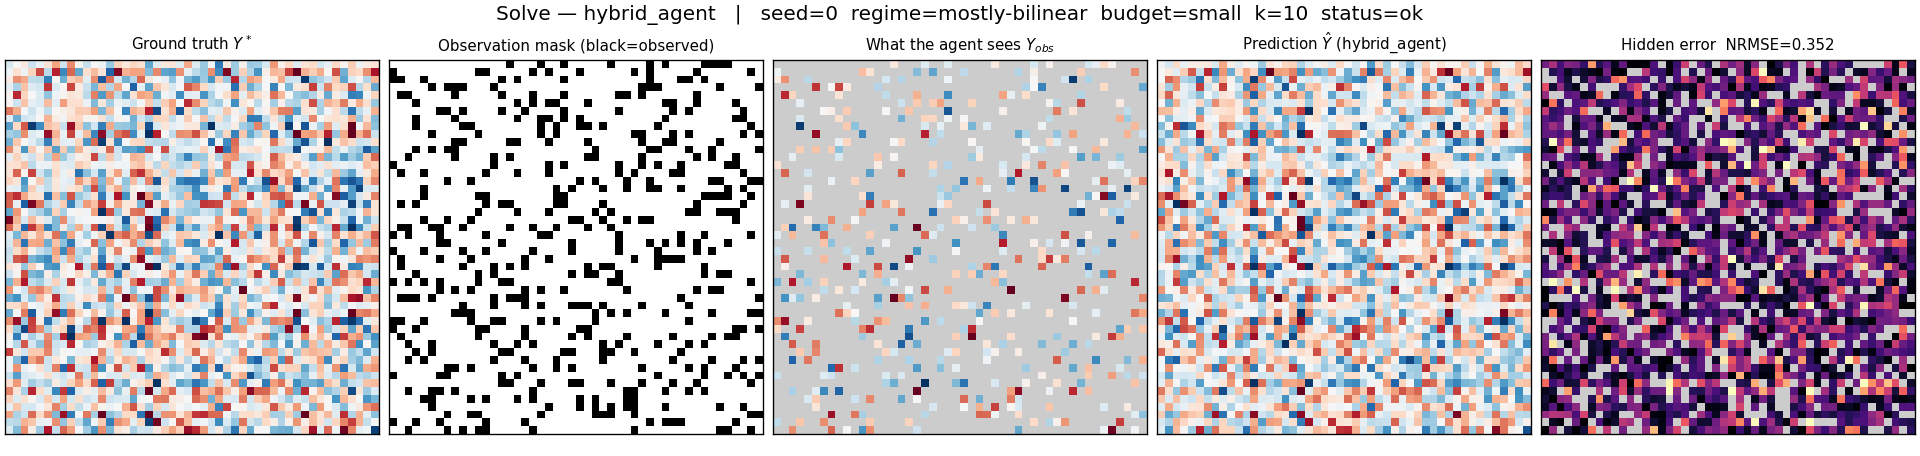
\includegraphics[width=\textwidth]{solve_hybrid_bilinear.png}
  \caption{Anatomy of a single reconstruction (the hybrid baseline on a
    bilinear-regime instance). From left to right: the hidden ground truth
    $Y^*$; the observation mask $M$ (observed cells in black); the masked input
    $Y^{\text{obs}}$ the agent actually receives (visible cells colored, hidden
    cells gray); the agent's prediction $\hat{Y}$; and the absolute error on the
    \emph{hidden} cells only --- the entries that count toward the score. Signed
    values use a diverging red/blue colormap centered at zero. These figures are
    produced by \texttt{scripts/visualize\_match.py} and are the standard way to
    read every example in this document.}
  \label{fig:solve-anatomy}
\end{figure}

% ============================================================
\section{Formal Problem Definition}
% ============================================================

\subsection{Shared instance}

For each seed $s$ and budget configuration $B$, the grader creates:

\begin{equation}
  (X, Z, Y^*) = \texttt{generate\_instance}(s, B)
\end{equation}

where $X \in \mathbb{R}^{n \times d}$, $Z \in \mathbb{R}^{m \times d}$,
$Y^* \in \mathbb{R}^{n \times m}$.

\subsection{Observation mask}

A valid mask $M \in \{0,1\}^{n \times m}$ satisfies:
\begin{align}
  \sum_{j=1}^{m} M_{ij} &= k \quad \forall i \in [n] \label{eq:row-sum}\\
  \sum_{i=1}^{n} M_{ij} &= k \quad \forall j \in [m] \label{eq:col-sum}
\end{align}
and the bipartite graph $G_M$ with row nodes $R_0,\ldots,R_{n-1}$, column nodes
$C_0,\ldots,C_{m-1}$, and edge $R_i$--$C_j$ iff $M_{ij}=1$ must be \emph{connected}.

\subsection{Observed matrix}

\begin{equation}
  Y^{\text{obs}}_{ij} = \begin{cases} Y^*_{ij} & \text{if } M_{ij} = 1 \\ 0 & \text{otherwise} \end{cases}
\end{equation}

\subsection{Participant input/output}

\textbf{Input to \texttt{solve}:} $X,\, Z,\, Y^{\text{obs}},\, M,\, B,\, s$

\textbf{Output of \texttt{solve}:} $\hat{Y} \in \mathbb{R}^{n \times m}$

\textbf{Input to \texttt{attack}:} $X,\, Z,\, k,\, B,\, s$ \quad (no access to $Y^*$)

\textbf{Output of \texttt{attack}:} a valid mask $M \in \{0,1\}^{n \times n}$

% ============================================================
\section{Matrix Generator}
% ============================================================

The ground-truth matrix is:

\begin{equation}
  Y^*_{ij} = w_{\text{bil}}\, \mathbf{x}_i^\top W \mathbf{z}_j
           + w_{\text{lat}}\, \mathbf{u}_i^\top \mathbf{v}_j
           + w_{\text{nl}} \sum_{\ell=1}^{r_{\text{nl}}} a_\ell \tanh\!\left((\mathbf{x}_i^\top \mathbf{p}_\ell)(\mathbf{z}_j^\top \mathbf{q}_\ell)\right)
           + \varepsilon_{ij}
  \label{eq:generator}
\end{equation}

where:
\begin{itemize}
  \item $W \in \mathbb{R}^{d \times d}$ is a random bilinear interaction matrix.
  \item $U \in \mathbb{R}^{n \times r}$, $V \in \mathbb{R}^{m \times r}$ give the latent low-rank term.
  \item $P \in \mathbb{R}^{d \times r_{\text{nl}}}$, $Q \in \mathbb{R}^{d \times r_{\text{nl}}}$,
        $a \in \mathbb{R}^{r_{\text{nl}}}$ define the nonlinear component.
  \item $\varepsilon_{ij} \sim \mathcal{N}(0, \sigma^2)$ is entry-level noise.
  \item $w_{\text{bil}}, w_{\text{lat}}, w_{\text{nl}}$ are regime-dependent mixture weights.
\end{itemize}

$Y^*$ is normalized to have zero mean and unit standard deviation after generation.

\subsection{Regimes}

The generator selects a \emph{regime} deterministically from the seed:

\begin{center}
\begin{tabular}{lcccc}
\toprule
Regime & $w_{\text{bil}}$ & $w_{\text{lat}}$ & $w_{\text{nl}}$ & $\sigma$ \\
\midrule
Mostly bilinear    & 0.85 & 0.10 & 0.05 & 0.05 \\
Mostly low-rank    & 0.10 & 0.85 & 0.05 & 0.05 \\
Mixed              & 0.45 & 0.45 & 0.10 & 0.05 \\
Nonlinear dominant & 0.25 & 0.25 & 0.50 & 0.10 \\
Noisy              & 0.60 & 0.30 & 0.10 & 0.20 \\
Spiky              & 0.40 & 0.40 & 0.20 & 0.05 \\
\bottomrule
\end{tabular}
\end{center}

In the spiky regime, a random subset of rows and columns receive feature vectors with
3× larger magnitude, creating high-leverage entries.

\begin{figure}[ht]
  \centering
  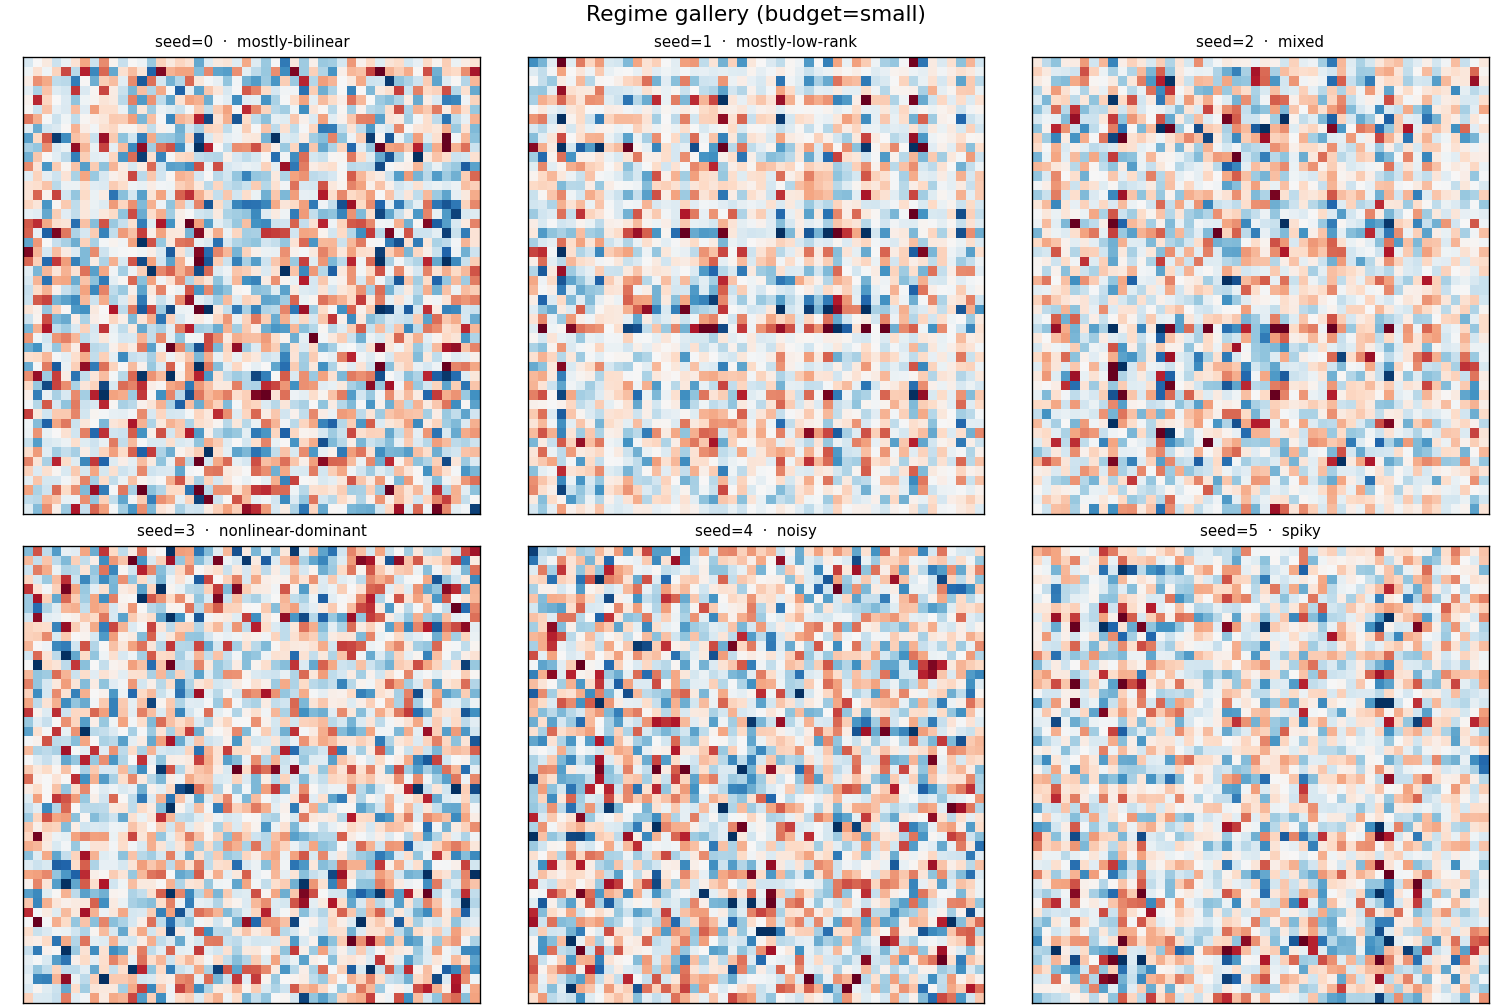
\includegraphics[width=\textwidth]{regime_gallery.png}
  \caption{One normalized ground-truth matrix $Y^*$ per generative regime
    (small budget, $48 \times 48$). The regimes differ in structure: the
    low-rank-dominant instance shows smoother row/column banding, while the
    bilinear, noisy, and nonlinear instances carry more high-frequency detail.
    A robust agent must perform well across all of them, since the regime is
    chosen deterministically from the hidden seed and is not revealed.}
  \label{fig:regime-gallery}
\end{figure}

% ============================================================
\section{Solve-Only Phase}
% ============================================================

Each agent is evaluated on a set of seeds using the \emph{official mask}
(a deterministic random $k$-regular connected mask generated by the grader).

The reconstruction loss on hidden entries is:

\begin{equation}
  \text{NRMSE}(\hat{Y}, Y^*, M) =
    \frac{\sqrt{\frac{1}{|\bar{M}|} \sum_{(i,j):\, M_{ij}=0} (\hat{Y}_{ij} - Y^*_{ij})^2}}
         {\text{std}(Y^*[\bar{M}]) + 10^{-8}}
  \label{eq:nrmse}
\end{equation}

where $\bar{M}$ denotes the complement of $M$ (hidden entries).

The instance-level solve score is:

\begin{equation}
  \text{SolveScore} = \log\!\left(\frac{\text{NRMSE}_{\text{mean}}}{\max(\text{NRMSE}_{\text{agent}},\, 10^{-12})}\right)
  \label{eq:solve-score}
\end{equation}

where $\text{NRMSE}_{\text{mean}}$ is the loss of the mean-fill baseline.
Scores are positive when the agent beats the baseline, zero if equal, negative if worse.

% ============================================================
\section{Arena Phase (Duels)}
% ============================================================

\subsection{Duel protocol}

A duel between agents $A$ and $B$ on seed $s$:

\begin{enumerate}
  \item Grader creates $(X, Z, Y^*)$ from seed $s$.
  \item $A$ generates mask $M_B$ for $B$: $M_B \leftarrow A.\texttt{attack}(X,Z,k,B,s_A)$.
  \item $B$ generates mask $M_A$ for $A$: $M_A \leftarrow B.\texttt{attack}(X,Z,k,B,s_B)$.
  \item Invalid masks are replaced by the official mask; the attacking agent receives penalty $\delta = 0.5$.
  \item $A$ solves under $M_A$: $\hat{Y}_A \leftarrow A.\texttt{solve}(X,Z,Y^{\text{obs}}_A,M_A,B,s)$.
  \item $B$ solves under $M_B$: $\hat{Y}_B \leftarrow B.\texttt{solve}(X,Z,Y^{\text{obs}}_B,M_B,B,s)$.
  \item Compute $L_A = \text{NRMSE}(\hat{Y}_A, Y^*, M_A) + \delta_A$ and $L_B$ similarly.
\end{enumerate}

\subsection{Outcome}

\begin{equation}
  \text{winner} = \begin{cases}
    A & \text{if } L_A < L_B\,(1-\varepsilon) \\
    B & \text{if } L_B < L_A\,(1-\varepsilon) \\
    \text{draw} & \text{otherwise}
  \end{cases}
  \qquad \varepsilon = 10^{-4}
  \label{eq:duel-outcome}
\end{equation}

\begin{figure}[ht]
  \centering
  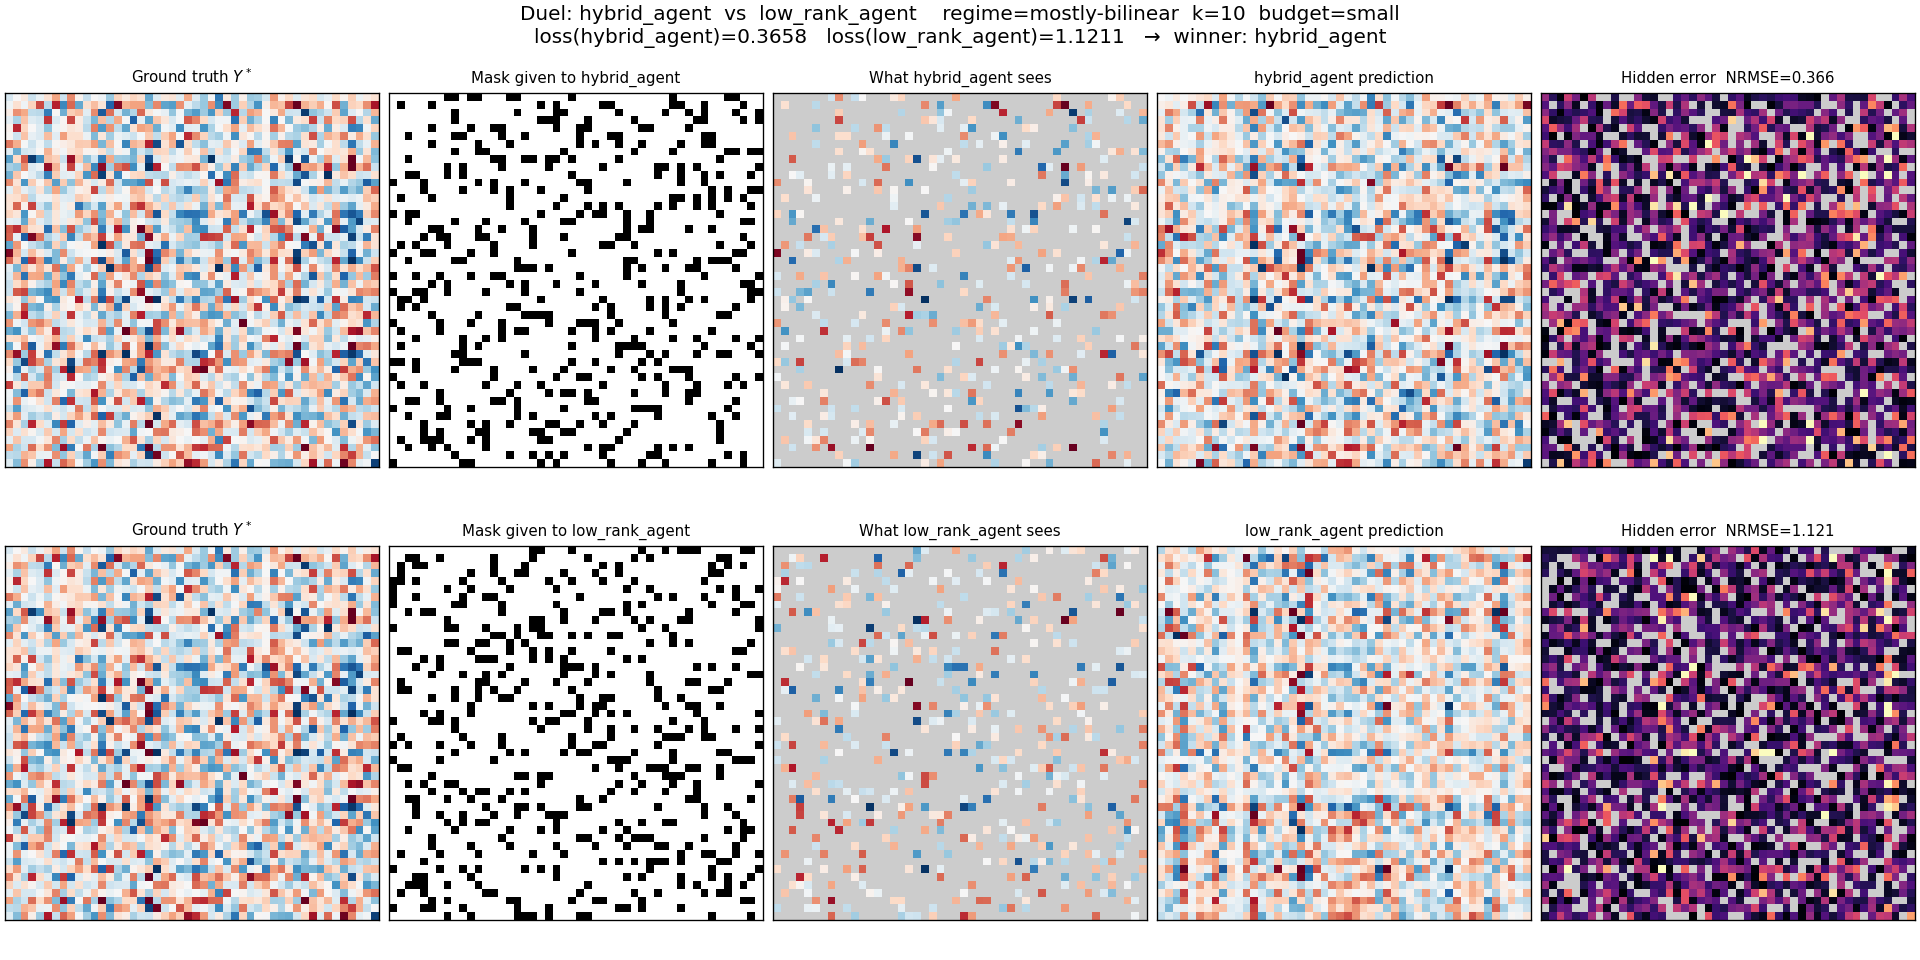
\includegraphics[width=\textwidth]{duel_hybrid_vs_lowrank.png}
  \caption{A duel (top row: hybrid baseline; bottom row: low-rank baseline).
    Both agents reconstruct the \emph{same} hidden matrix $Y^*$ (identical
    leftmost panels), but each receives a \emph{different} observation mask
    chosen by its opponent (second column) --- so each sees a different subset
    of the matrix (third column). Comparing the rightmost hidden-error panels
    settles the duel: the hybrid agent's error is markedly lower
    (NRMSE $\approx 0.37$ vs.\ $\approx 1.12$), so it wins per
    Eq.~\eqref{eq:duel-outcome}. Read each row using the panel layout of
    Figure~\ref{fig:solve-anatomy}.}
  \label{fig:duel}
\end{figure}

% ============================================================
\section{Ranking}
% ============================================================

\subsection{Arena points}

\begin{equation}
  \text{ArenaPoints}_i = \frac{W_i + \tfrac{1}{2} D_i}{W_i + D_i + L_i}
\end{equation}

where $W_i$, $D_i$, $L_i$ are total wins, draws, and losses for agent $i$.

\subsection{Bradley-Terry rating}

The Bradley-Terry model assigns skill parameters $r_i$ such that:

\begin{equation}
  P(i \text{ beats } j) = \frac{e^{r_i}}{e^{r_i} + e^{r_j}}
  \label{eq:bradley-terry}
\end{equation}

Parameters are fit by the MM algorithm on observed win/draw counts.
Draws count as $\tfrac{1}{2}$ win for each side. Ratings are normalized to zero mean.

Elo-like conversion:

\begin{equation}
  \text{Elo}_i = 1500 + \frac{400}{\ln 10} \cdot r_i
\end{equation}

\subsection{Final score}

\begin{equation}
  \text{FinalScore}_i = 0.60 \cdot \widetilde{S}_i + 0.35 \cdot \widetilde{E}_i + 0.05 \cdot R_i
  \label{eq:final-score}
\end{equation}

where $\widetilde{S}_i$ is min-max normalized solve score, $\widetilde{E}_i$ is min-max
normalized Elo, and $R_i \in [0,1]$ is a robustness score that penalizes crashes,
invalid masks, timeouts, and NaN/Inf outputs.

If $\max = \min$ during normalization, all agents receive $0.5$.

% ============================================================
\section{Budget Levels}
% ============================================================

\begin{center}
\begin{tabular}{lccccccc}
\toprule
Level  & $n$ & $m$ & $d$ & $r$ & $r_{\text{nl}}$ & $k$ & Solve timeout \\
\midrule
small  & 48  & 48  & 12 & 4  & 2  & 10 & 1.0\,s  \\
medium & 96  & 96  & 24 & 8  & 4  & 12 & 5.0\,s  \\
large  & 160 & 160 & 32 & 12 & 6  & 16 & 15.0\,s \\
\bottomrule
\end{tabular}
\end{center}

Default weighting across budget levels: small 30\%, medium 45\%, large 25\%.

Public grader uses \textbf{small} and \textbf{medium} only.
Hidden grader includes \textbf{large}.

% ============================================================
\section{Participant API}
% ============================================================

Participants submit a single Python file defining:

\begin{lstlisting}
class Agent:
    def solve(self, X, Z, Y_obs, mask, budget, seed):
        """
        X      : np.ndarray (n, d)  -- row features
        Z      : np.ndarray (m, d)  -- column features
        Y_obs  : np.ndarray (n, m)  -- observed entries (0 where hidden)
        mask   : np.ndarray (n, m), bool  -- True where observed
        budget : dict  -- config info
        seed   : int

        Returns
        -------
        Y_hat  : np.ndarray (n, m)
        """

    def attack(self, X, Z, k, budget, seed):
        """
        Returns
        -------
        mask : np.ndarray (n, n), bool
               k-regular, connected bipartite adjacency matrix
        """
\end{lstlisting}

\paragraph{The \texttt{seed} argument is decoupled from the instance.}
The \texttt{seed} passed to \texttt{solve} and \texttt{attack} exists only so
that an agent's own randomness can be made deterministic. It is \emph{not} the
seed used to generate the instance: the grader derives it from the (private)
generation seed through a one-way function, and the graded evaluation draws
secret, high-entropy generation seeds that are never exposed. Consequently an
agent cannot rebuild $Y^*$ by calling the public generator on \texttt{seed}, nor
by brute-forcing which generation seed reproduces the fully-visible $X$. Such
attempts fail on the real grader --- they produce an unrelated matrix --- and
merely waste the agent's time budget.

% ============================================================
\section{Validity and Robustness Constraints}
% ============================================================

\subsection{Valid predictions}

A prediction $\hat{Y}$ is valid if:
\begin{itemize}
  \item Shape equals $(n, m)$.
  \item All entries are finite ($|\hat{Y}_{ij}| \leq 10^5$).
  \item No NaN or Inf values.
\end{itemize}

Invalid predictions receive $\text{NRMSE} = 10^6$.

\subsection{Valid masks}

A mask $M$ is valid if it satisfies equations \eqref{eq:row-sum}--\eqref{eq:col-sum}
and the induced bipartite graph is connected. Invalid masks receive a penalty of
$\delta = 0.5$ added to the attacking agent's final loss for that duel.

\subsection{Timeouts}

Agents exceeding \texttt{solve\_timeout\_s} or \texttt{attack\_timeout\_s} are
penalized as if they returned an invalid result.

\subsection{Fair play: no instance reconstruction}

The task is to \emph{predict} the hidden entries, not to recover the instance.
The following are forbidden and do not work against the graded evaluation:
\begin{itemize}
  \item Rebuilding $Y^*$ by calling the public generator on the provided
        \texttt{seed} (the seed is decoupled; see the Participant API section).
  \item Recovering the generation seed by brute-forcing which seed reproduces
        the visible $X$ (the graded evaluation uses secret, high-entropy
        generation seeds, so the search space is intractable).
  \item Reading $Y^*$ out of the grader's process memory. The hidden grader runs
        each agent in an isolated subprocess.
\end{itemize}
Agents must use only their declared inputs ($X$, $Z$, $Y^{\text{obs}}$, $M$,
\texttt{budget}, \texttt{seed}) to form a prediction.

% ============================================================
\section{Suggested Tactics}
% ============================================================

\subsection{Reconstruction (solve)}

\begin{enumerate}
  \item \textbf{Mean baseline}: fill all hidden entries with the observed mean.
        Serves as the scoring reference.
  \item \textbf{Row/column means}: use per-row and per-column averages.
  \item \textbf{Ridge regression}: construct features
        $\phi_{ij} = [\mathbf{x}_i,\, \mathbf{z}_j,\, \mathbf{x}_i \odot \mathbf{z}_j]$
        and fit $Y_{ij} \approx \phi_{ij}^\top w$ via ridge regression.
  \item \textbf{Bilinear regression}: directly fit $\hat{Y} = X W Z^\top$
        by minimizing the observed MSE over $W$.
  \item \textbf{Low-rank factorization}: fit $\hat{Y} \approx P Q^\top$
        via alternating least squares (ALS) or gradient descent.
  \item \textbf{Hybrid}: combine bilinear and low-rank components.
  \item \textbf{PyTorch optimization}: use Adam or L-BFGS on a differentiable objective
        combining all terms (bilinear + low-rank + optional nonlinear).
  \item \textbf{Ensembling}: average predictions across multiple ranks and regularization strengths.
  \item \textbf{Early stopping}: hold out a subset of observed entries for validation.
  \item \textbf{Robust normalization}: center and scale predictions to match observed statistics.
\end{enumerate}

Note: the nonlinear component ($\tanh$) is \emph{weak and restricted} with at most
$r_{\text{nl}} \leq 6$ terms. The task is robust prediction, not exact nonlinear recovery.

\subsection{Adversarial mask design (attack)}

\begin{enumerate}
  \item \textbf{Random regular}: simplest valid attack. Provides no advantage but satisfies all constraints.
  \item \textbf{Low-leverage observation}: compute row leverage scores from $X$
        and column leverage scores from $Z$. Force the opponent to observe entries
        in low-leverage feature regions, where extrapolation is harder.
  \item \textbf{Minimum spanning tree mask}: design a mask whose bipartite observation
        graph is a spanning tree (minimal connectivity). This minimizes information
        flow while remaining valid.
  \item \textbf{Feature-antipodal mask}: place observations where
        $\mathbf{x}_i \approx -\mathbf{x}_{i'}$ and $\mathbf{z}_j \approx -\mathbf{z}_{j'}$,
        forcing sign symmetry ambiguities.
  \item \textbf{Diagonal avoidance}: avoid placing observations along the bilinear diagonal
        $X W Z^\top$ to prevent easy rank-1 recovery.
\end{enumerate}

% ============================================================
\section{Reproducibility and Deterministic Grading}
% ============================================================

All randomness is controlled by explicit seeds via \texttt{numpy.random.default\_rng}.
There is no global random state. Running the grader twice on the same instances
produces identical results.

The grader separates two seeds. The \emph{generation seed} builds
$(X, Z, Y^*)$ and is private to the grader; in the graded evaluation it is drawn
with high entropy and never exposed. The \emph{agent seed} passed to
\texttt{solve}/\texttt{attack} is a one-way-derived value, decoupled from the
generation seed, provided solely so an agent's own randomness can be
deterministic. Participants must ensure their agents are deterministic given the
same agent seed; non-deterministic outputs are detected and penalized.

% ============================================================
\section{Baselines}
% ============================================================

The following reference baselines are provided in the \texttt{baselines/} directory:

\begin{itemize}
  \item \textbf{mean\_agent}: fills all hidden entries with the observed mean.
        Used as the scoring reference in equation~\eqref{eq:solve-score}.
  \item \textbf{ridge\_agent}: ridge regression on $[\mathbf{x}_i, \mathbf{z}_j, \mathbf{x}_i \odot \mathbf{z}_j]$.
  \item \textbf{low\_rank\_agent}: ALS matrix factorization $\hat{Y} \approx P Q^\top$.
  \item \textbf{hybrid\_agent}: bilinear term $X W Z^\top$ plus low-rank ALS residual.
  \item \textbf{random\_attack\_agent}: mean-fill solve with a random-regular attack mask.
\end{itemize}

A positive solve score requires beating the mean baseline.
The competition leaderboard normalizes scores relative to all submitted agents and baselines.

% ============================================================
\section{Submission Instructions}
% ============================================================

\noindent\textbf{Deadline.} The final day for submissions is
\textbf{July 5, 2026} (end of day, Yerevan time). You may resubmit any number of
times before the deadline; the latest valid submission is the one that counts.

\begin{enumerate}
  \item Copy \texttt{examples/agent\_template.py} to a new file, e.g.\ \texttt{my\_agent.py}.
  \item Implement \texttt{solve()} and \texttt{attack()}.
  \item Test locally:
    \begin{lstlisting}
python scripts/run_public_grader.py \
    --agents my_agent.py --seeds 20
    \end{lstlisting}
  \item Verify your agent is valid:
    \begin{lstlisting}
pytest tests/ -v
    \end{lstlisting}
  \item Submit \texttt{my\_agent.py} to the competition portal.
\end{enumerate}

Your submission must:
\begin{itemize}
  \item Define exactly one class named \texttt{Agent} with both \texttt{solve} and \texttt{attack} methods.
  \item Not read from or write to the filesystem during evaluation.
  \item Not rely on shared mutable state between calls.
  \item Return valid \texttt{numpy} arrays of the correct shape and dtype.
\end{itemize}

\end{document}
